\chapter{Methodology}
To achieve the swing up task, we employ the classical model-free reinforcement learning algorithm known as Soft actor critic to train a policy which is able to reach the region of attraction(RoA) of a continuous time linear quadratic regulator(LQR) controller. As soon as the system enters the RoA, we transition to the LQR controller to stabilize the entire system.

\section{Soft actor critic}
Soft Actor Critic (SAC) is a popular algorithm
used in the field of reinforcement learning. It is originally
designed for continuous action spaces, where the agent has
an infinite choice of actions to take. In our problem scenario,
the actuators of the double pendulum can be set to any
value within the torque limit range. The position and velocity
measurements obtained from the motors are also represented
as continuous real numbers. Therefore, we choose the SAC algorithm to train the agent.

SAC optimizes a policy by maximizing the expected cumulative reward obtained by
the agent over time. This is achieved through an actor and critic
structure.

The actor is responsible for selecting actions based on the current policy in
response to the observed state of the environment. It is typically represented
by a shallow neural network that approximates the mapping between the input
state and the output probability distribution over actions. SAC incorporates a
stochastic policy in its actor part, which encourages exploration and helps the
agent improve policies.

The critic, on the other hand, evaluates the value of state-action pairs. It
estimates the expected cumulative reward that the agent can obtain by following
a certain policy. Typically, the critic is also represented by a neural
network that takes state-action pairs as inputs and outputs estimated value.

In addition to the actor and critic, a central feature of SAC is entropy
regularization. The policy is trained to maximize a trade-off between expected return and entropy, which is a measure of randomness in the action selection. If
\(x\) is a random variable with a probability density function \(P\), the
entropy \(H\) of \(x\) is defined as:

\[
 H(P) = \displaystyle \mathop{\mathbb{E}}_{x \sim P}[-\log P(x)]
\]

By maximizing entropy, SAC encourages exploration and accelerates learning. It
also prevents the policy from prematurely converging to a suboptimal solution.
The trade-off between maximizing reward and maximizing entropy is controlled
through a parameter, \(\alpha\). This parameter serves to balance the importance
of exploration and exploitation within the optimization problem. The optimal policy
\(\pi^*\) can be defined as follows:

\[
 \pi^* = {arg}{\max_{\pi}}{\displaystyle
 \mathop{\mathbb{E}}_{\tau\sim\pi}}{\Bigg[{\sum_{t=0}^{\infty}}{\gamma^{t}}{\Big(R(s_t,a_t,s_{t+1})}+{\alpha}H(\pi(\cdot\mid{s_t}))\Big)\Bigg]}
\]

During training, SAC learns a policy $\pi_{\theta}$ and two Q-functions
$Q_{\phi_1} , Q_{\phi_2}$ concurrently. The loss functions for the two Q-networks are
$(i \in {1, 2})$:

\[
  L(\phi_i,D) = \displaystyle
  \mathop{\mathbb{E}}_{(s,a,r,s',d)\sim{D}}\bigg[\bigg(Q_{\phi_i}(s,a)-y(r,s',d)\bigg)^2\bigg],
\]

where the temporal difference target \(y\) is given by:
\begin{align*}
  y(r,s',d) &= r + \gamma(1-d) \times \nonumber \\
  & \bigg(\displaystyle
  \mathop{\min}_{j=1,2}Q_{\phi_{targ,j}}(s',\tilde{a}')-\alpha\log
  {\pi_\theta}(\tilde{a}'\mid{s}')\bigg), \\
  \tilde{a}'&\sim{\pi_\theta}(\cdot\mid{s'})
\end{align*}

In each state, the policy \(\pi_\theta\) should act to maximize the expected
future return \(Q\) while also considering the expected future entropy \(H\). In other
words, it should maximize \(V^\pi(s)\):
\begin{align*}
 V^\pi(s) &= {\displaystyle \mathop{\mathbb{E}}_{a\sim\pi}[Q^\pi(s,a)]} +
 \alpha{H(\pi(\cdot\mid{s}))} \\
 &= {\displaystyle \mathop{\mathbb{E}}_{a\sim\pi}[Q^\pi(s,a)]} -
 \alpha{\log {\pi(a\mid{s})}}
\end{align*}


By employing an effective gradient-based optimization technique, the parameters
of both the actor and critic neural networks undergo updates, subsequently
leading to the adaptation of the policies themselves.

In conclusion, SAC's combination of stochastic policies, exploration through
entropy regularization, value estimation, and gradient-based optimization make
it a well-suited algorithm for addressing the challenges posed by continuous
state and action spaces.

\section{Linear quadratic regulator}
We have the general form of a nonlinear system:
\begin{equation}
    \dot{x}(t) = f(x(t), u(t))
\end{equation}

Linearize it around an operating point:
\begin{equation}
    \dot{\overline{x}}(t) = A \overline{x}(t) + B u(t)
\end{equation}

The difference of the current state and the desired state is:
\begin{equation}
    \overline{x} = x - x_{\text{op}}, \quad \dot{\overline{x}} = \dot{x}
\end{equation}

where \(A\) and \(B\) can be calculated as:
\begin{equation}
    A = \left.\frac{\partial f}{\partial x}\right|_{\text{op}}, \quad B = \left.\frac{\partial f}{\partial u}\right|_{\text{op}}
\end{equation}

The cost function we are dealing with here is:
\begin{equation}
J = \int_0^{\infty} \left( x^T Q x + u^T R u \right) dt
\end{equation}

Based on the Riccati equation:
\begin{equation}
    A^T S + SA - SBR^{-1}B^T S + Q = 0
\end{equation}

 the LQR control law for the linearized system:
\begin{equation}
    u(t) = -K\overline{x}(t)
\end{equation}

Where \(K\) can be calculated as:
\begin{equation}
    K = R^{-1}B^T S
\end{equation}

\section{Combining SAC and LQR with region of attraction}
This section is about how to use ROA to combine SAC and LQR

How to optimize the RoA of the LQR controller

First, construct Lyapunov function for stability check:
\begin{equation}
    0< V(\bar{x}) = \bar{x}^T S \bar{x} < \rho
\end{equation}

Second, first derivative of Lyapunov function has to be negative
\begin{equation}
    \dot{V}(\bar{x}) = 2\dot{\bar{x}}^T S \bar{x} < 0
\end{equation}

Choose suitable \(\rho\) and \(S\) that maximize the volumn of an ellipsoid shaped RoA in 4D state space.

\begin{figure}[htbp]
    \centering
    \includegraphics[width=0.6\textwidth]{example-image.png} % Adjust the width as needed
    \caption{Region of Attraction}
    \label{fig:example}
\end{figure}

\section{Reward shaping}
This section is about the reward shaping problem of reinforcement learning training.

\begin{equation}
\begin{aligned}
 r(x,u) = &-(x - x_g)^T Q_{train} (x - x_g) - u^T R_{train}u \nonumber\\
           & +
            \begin{dcases*}
              r_{line} & \text{if} $h(p_1, p_2) \geq h_{line}$\, ,\\
              0 & \text{else}
            \end{dcases*}\nonumber\\
           & +
            \begin{dcases*}
              r_{LQR} & \text{if} $(x - x_g)^T S_{LQR} (x - x_g) \geq \rho $\, ,\\
              0 & \text{else}
            \end{dcases*}\nonumber\\
           & -
            \begin{dcases*}
              r_{vel} & \text{if} $|v_1| \geq v_{thresh}$\, ,\\
              0 & \text{else}
            \end{dcases*}\nonumber\\
           & -
            \begin{dcases*}
              r_{vel} & \text{if} $|v_2| \geq v_{thresh}$\, ,\\
              0 & \text{else}
            \end{dcases*}
\end{aligned}
\end{equation}

\begin{figure}[htbp]
    \centering
    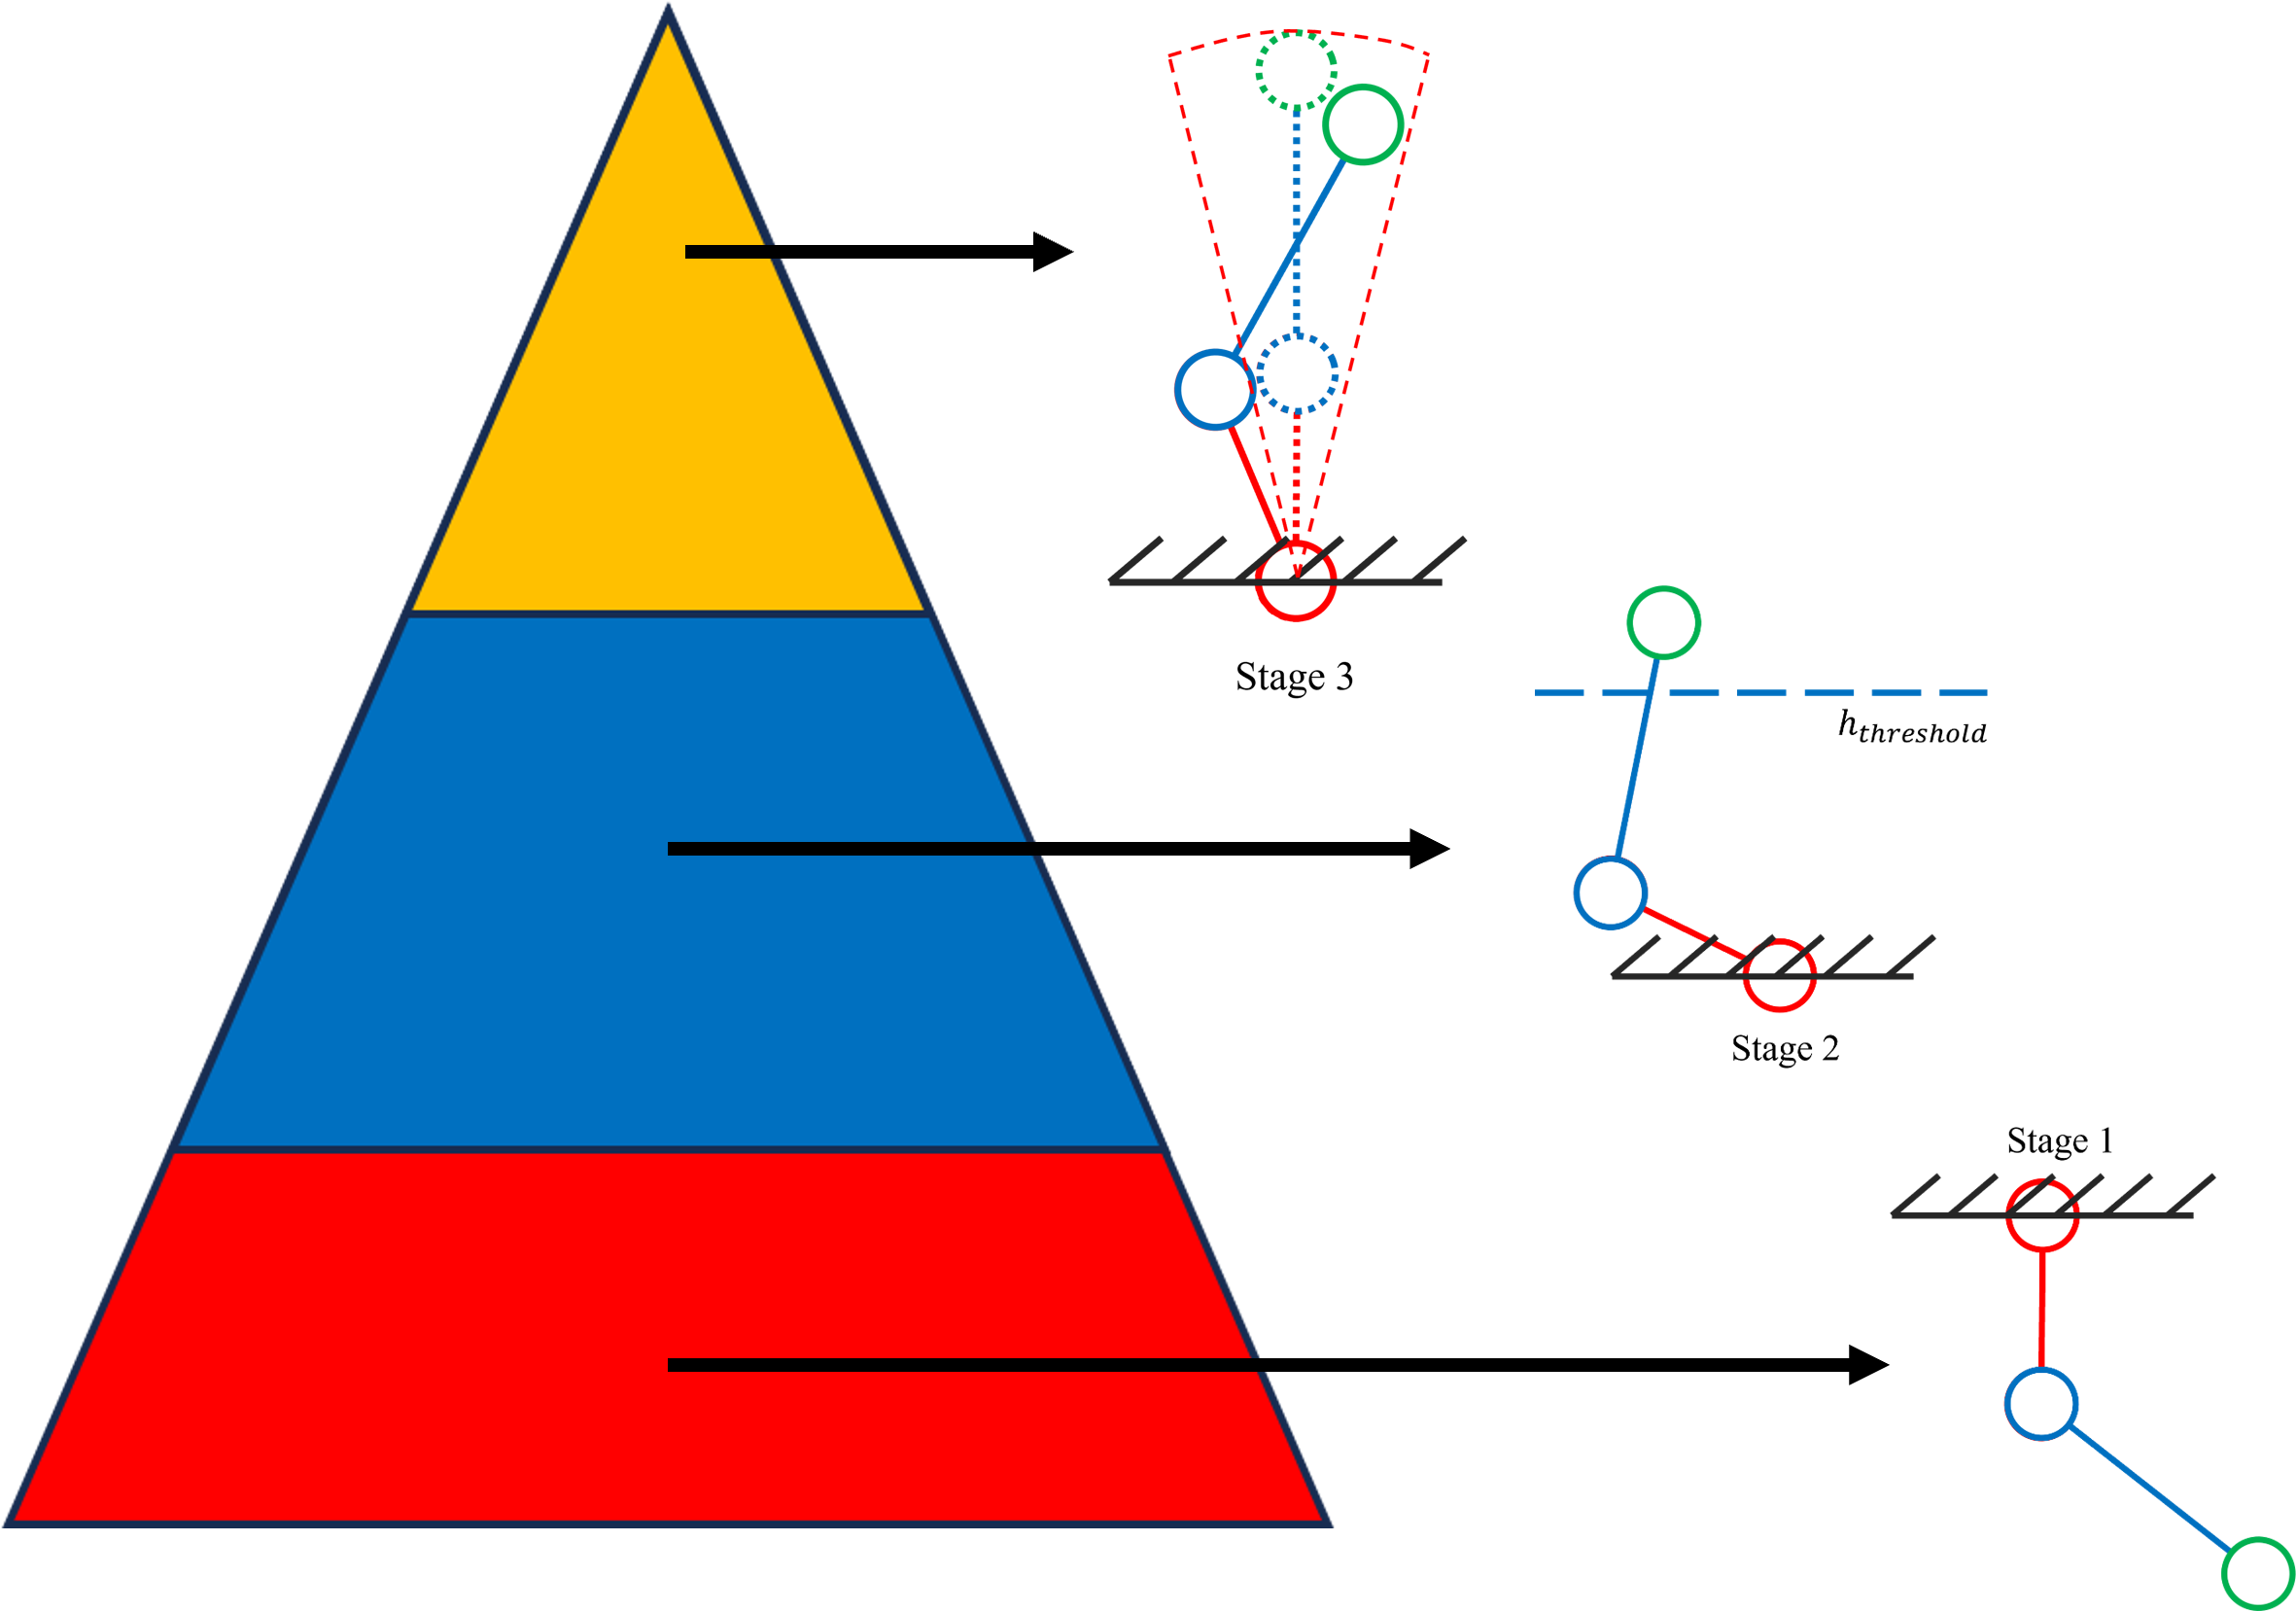
\includegraphics[width=0.9\textwidth]{figures/reward_explained.png} % Adjust the width as needed
    \caption{Interpretation of reward shaping}
    \label{fig:example}
\end{figure}

\cleardoublepage
